\section[Algorithme du Perceptron]{Algorithme du Perceptron}

\subsection[Historique]{Historique}

\begin{frame}{Historique}
	\begin{itemize}
		\item \textbf{1943}: McCulloch (neurophysiologiste) et Pitts (mathématicien) établissent le premier modèle mathématique d'un \textbf{neurone humain}. C'est un modèle binaire et purement logique. Les paramètres sont fixés manuellement. Ils cherchent à montrer que le cerveau humain est une machine à calculer et montrent comment programmer des portes logiques (ET, OU, NON) avec ce modèle.
		\pause
		\item \textbf{1948}: Hebb (neuropsychologue) a été le premier à émettre l'hypothèse que le cerveau était plastique. A l'époque on pensait que les connexions entre les neurones étaient établies une fois pour toutes à la naissance. Il théorise donc que les connexions entre neurones se renforcent durant l'apprentissage: \textit{"Des neurones qui s'activent ensemble se connectent ensemble."}
		\item \textbf{1958}: Rosenblatt (psychologue) s'inspire des travaux de Hebb pour améliorer la vision de McCulloch et Pitts. Il a l'idée de mettre à jour les paramètres du neurone mathématique en fonction de l'erreur commise par ce même neurone. Il invente le premier algorithme d'apprentissage: le Perceptron.
	\end{itemize}
\end{frame}

\begin{frame}{Historique}
	\begin{itemize}
		\item \textbf{1969}: Minsky et Papert démontrent formellement que l'algorithme du Perceptron ne permet pas de programmer une porte OU exclusif. Ils montrent aussi qu'il faudrait en fait plusieurs neurones pour programmer une telle porte mais que l'algorithme d'apprentissage ne marchait plus dans ce cas. Cela met un terme à la recherche sur le Perceptron.
		\pause 
		\item \textbf{1986}: Rumelhart, Hinton et Williams publient un article qui présente l'algorithme de rétro-propagation du gradient qui permet d'entraîner un Perceptron multicouche. Ils arrivent à entraîner un réseau de neurones qui réplique une porte logique OU exclusif. D'autres scientifiques apportent des contributions antérieures à cet article: Linnainmaa (1970), Werbos (1974) et Le Cun (1985).
	\end{itemize}
\end{frame}

\subsection[Intuition du Perceptron]{Intuition du Perceptron}

\begin{frame}{Approche géométrique}
	Dans un plan défini par les variables $X_1$ et $X_2$, l'équation d'une droite $\mathcal{D}$ est donnée par:
	
	\begin{equation*}
		w_1 \cdot x_1 + w_2 \cdot x_2 + w_3 = 0
	\end{equation*}
	
	\vspace{0.3cm}
	
	Avec $w_1$, $w_2$ et $w_3$, les coefficients de la droite.

	\begin{figure}
		\centering
		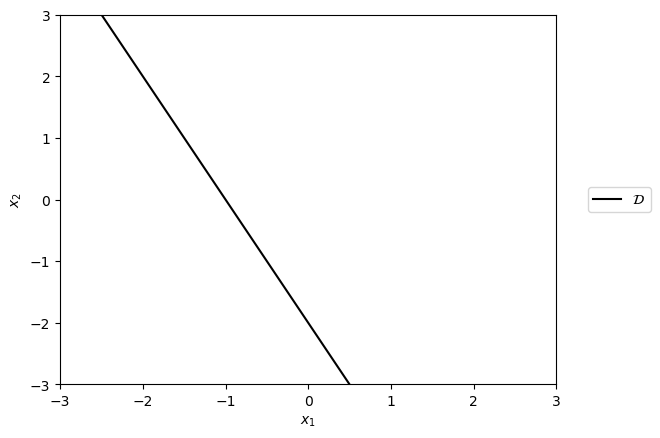
\includegraphics[height=0.3\linewidth]{Images/droite01}
		\label{fig:droite01}
	\end{figure}			

\end{frame}

\begin{frame}{Régions de l'espace}
	On nomme $z$ la quantité suivante:
	
	\begin{equation*}
		z = w_1 \cdot x_1 + w_2 \cdot x_2 + w_3
	\end{equation*}
	
	La droite $\mathcal{D}$ \textbf{sépare} l'espace en deux régions distinctes:
	
	\begin{itemize}
		\item Une région pour laquelle $z > 0$.
		\item Une région pour laquelle $z < 0$.
	\end{itemize}
	
	\vspace{0.2cm}
	
	Sur la droite $\mathcal{D}$, $z$ est par définition nulle.

	\begin{figure}
		\centering
		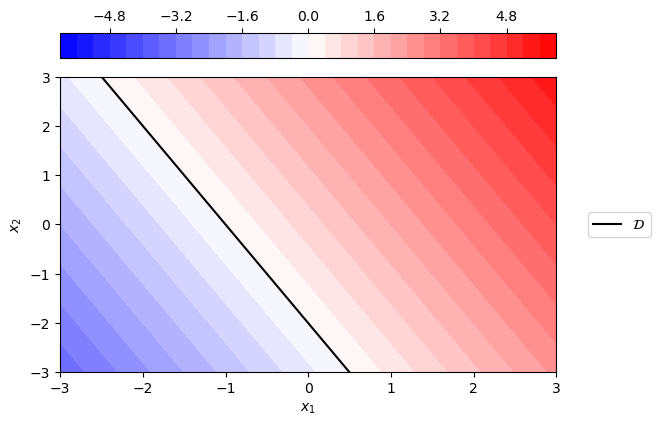
\includegraphics[height=0.3\linewidth]{Images/droite02}
		\label{fig:droite02}
	\end{figure}
	
\end{frame}

\begin{frame}{Position d'un point}
	On note $P$, un point de coordonnées $\left( x_1^{(P)}, x_2^{(P)} \right)$:
				
	\begin{equation*}
		z^{(P)} = w_1 \cdot x_1^{(P)} + w_2 \cdot x_2^{(P)} + w_3
	\end{equation*}
	
	\begin{figure}
		\centering
		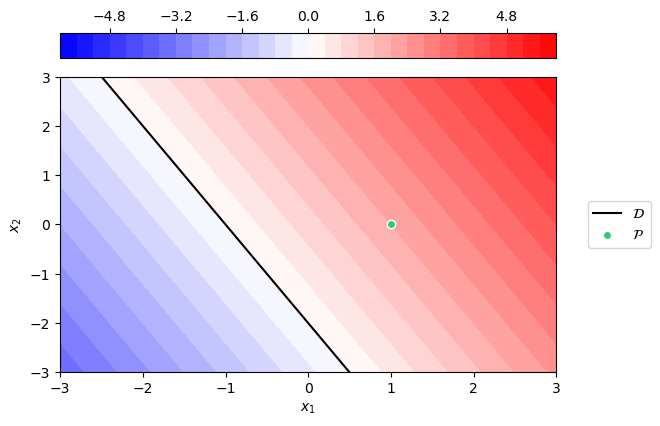
\includegraphics[height=0.4\linewidth]{Images/droite03}
		\label{fig:droite03}
	\end{figure}
\end{frame}

\begin{frame}{Problème de classification}
	Dans un problème de classification binaire \textbf{linéairement séparable}:
	
	\begin{itemize}
		\item On dispose de plusieurs points: $\mathcal{P} = \left\{ \left( x_1^{(i)}, x_2^{(i)}\right) \right\}_{i=1}^n$.
		\item Chaque point (ou observation) est associé à une classe $K = \{0, 1\}$.
		\item On cherche alors une droite $\mathcal{D}$ \textbf{séparant parfaitement} les observations des deux classes.
	\end{itemize}
	
	\vspace{0.3cm}
	\pause
	
	Cela revient à trouver une droite $\mathcal{D}$ telle que \textit{toutes} les observations de la classe $K = 1$ aient une quantité $z$ \textbf{positive} et que \textit{toutes} les observations de la classe $K = 0$ aient une quantité $z$ \textbf{négative}.
	
	\vspace{0.3cm}
	\pause
	
	Pour simplifier l'écriture de l'algorithme du Perceptron, on considèrera des données \textbf{augmentées} pour $x$:
	
	\begin{equation*}
		x^{(i)} = \left( x_1^{(i)}, x_2^{(i)}, 1\right)
	\end{equation*}
\end{frame}

\begin{frame}{Algorithme du Perceptron de Rosenblatt}
	Pour un problème de classification binaire linéairement séparable:
	\begin{enumerate}
		\item On initialise aléatoirement les coefficients $w_1$, $w_2$, $w_3$.
		\pause
		\item Boucle principale: \textbf{epochs}
		\pause
		\begin{itemize}
			\item Pour chaque observation $i$:
			\begin{itemize}
				\item On calcule la quantité $z^{(i)} = w_1 \cdot x_1^{(i)} + w_2 \cdot x_2^{(i)} + w_3 \cdot 1$.
				\pause
				\item On calcule le signe de cette quantité, que l'on notera $\sign{z^{(i)}}$:
				\begin{equation*}
					\sign{z^{(i)}} = 
					\begin{cases}
						1 & \text{si} \; z^{(i)} \ge 0 \\
						0 & \text{sinon}
					\end{cases}
				\end{equation*}
				\item On compare $\sign{z^{(i)}}$ à la classe $y^{(i)}$ et on ajuste avec un taux d'apprentissage $\alpha \in \mathbb{R}$ faible, pour tout $j = 1, 2, 3$:
				\begin{equation*}
					w_j \leftarrow w_j + \alpha \cdot \left[y^{(i)} - \sign{z^{(i)}}\right] \cdot x_j^{(i)}
				\end{equation*}
			\end{itemize}
			\pause
			\item On répète jusqu'à ce que toutes les observations aient été traitées.
		\end{itemize}
		\pause
		\item On répète l'étape 2 jusqu'à ce que toutes les observations soient bien classées: $\operatorname{sign}(z^{(i)}) = y^{(i)} \; \forall \; i=1, 2, \cdots n$.
	\end{enumerate}
\end{frame}

\begin{frame}{Interprétation géométrique de l'algorithme du Perceptron}
	Supposons que nous avons une observation $i$ telle que $y^{(i)} = 0$ et $z^{(i)} > 0$. Comme le signe de $z$ ne correspond pas à la classe vraie, l'algorithme du Perceptron effectue une mise à jour depuis l'état $k$ des coefficient de la droite:
	
	\begin{equation*}
		\begin{aligned}
			w_j^{(k+1)} 
			&= w_j^{(k)} + \alpha \cdot \left[ y^{(i)} - \sign{z^{(i)}}\right] \cdot x_j^{(i)} \\
			&= w_j^{(k)} - \alpha \cdot x_j^{(i)}
		\end{aligned}
	\end{equation*}
	
	\begin{figure}
		\centering
		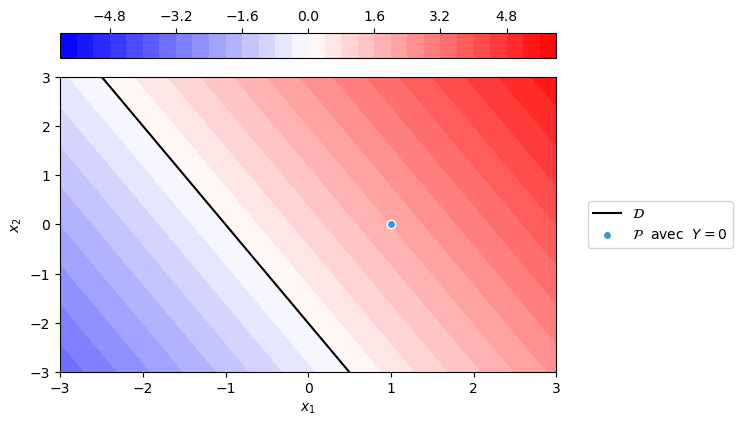
\includegraphics[height=0.3\linewidth]{Images/droite04}
		\label{fig:droite04}
	\end{figure}	
	
\end{frame}

\begin{frame}{Interprétation géométrique de l'algorithme du Perceptron}
	En arrangeant les coefficients $w_j$ de la droite dans un vecteur colonne $w \in \mathcal{M}_{3,1}(\R)$ tel que $w = \begin{pmatrix}
		w_1 & w_2 & w_3
	\end{pmatrix}^T$, on a alors:
	
	\begin{equation*}
		\left(z^{(i)}\right)^{(k)} = x^{(i)}  w^{(k)}
	\end{equation*}
	
	Et:
	
	\begin{equation*}
		\begin{aligned}
			\left(z^{(i)}\right)^{(k+1)} 
			&= x^{(i)} w^{(k+1)} \\
			&= x^{(i)} \left[w^{(k)} - \alpha \left(x^{(i)}\right)^T\right] \\
			&= x^{(i)} w^{(k)} - \alpha x^{(i)} \left(x^{(i)}\right)^T \\
			&= \left(z^{(i)}\right)^{(k)} - \alpha \| x^{(i)} \|_2^2
		\end{aligned}
	\end{equation*}
	
\end{frame}

\begin{frame}{Interprétation géométrique de l'algorithme du Perceptron}
	Or:
	
	\begin{equation*}
		\alpha \| x^{(i)} \|_2^2 > 0
	\end{equation*}	
	
	Donc:
	
	\begin{equation*}
		\left(z^{(i)}\right)^{(k+1)} < \left(z^{(i)}\right)^{(k)}
	\end{equation*}
	
	\begin{itemize}
		\item La droite se déplace de telle sorte que la quantité $z$ diminue. La droite $\mathcal{D}$ se rapproche du point représentant l'observation, puis le dépasse de telle sorte qu'il se retrouve dans une zone pour laquelle $z^{(i)} < 0$.
		\item Lorsqu'il y a plusieurs observations, la droite doit se déplacer \textit{relativement} doucement pour ne pas dégrader trop le positionnement des autres points par rapport à la droite: $\alpha$ doit être suffisamment faible pour la stabilité de l'algorithme.
	\end{itemize}
	

\end{frame}

\begin{frame}{Application aux portes logiques ET et OU}
	\begin{columns}
		\begin{column}{0.5\textwidth}
			\begin{figure}
				\centering
				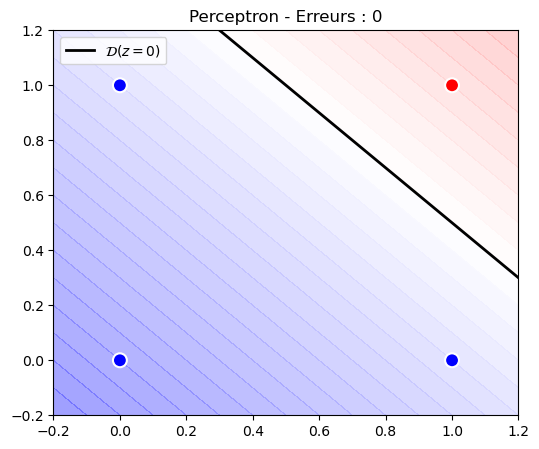
\includegraphics[height=0.8\linewidth]{Images/droite05}
				\label{fig:droite05}
				\caption*{Porte ET}
			\end{figure}			
		\end{column}
		\begin{column}{0.5\textwidth}
			\begin{figure}
				\centering
				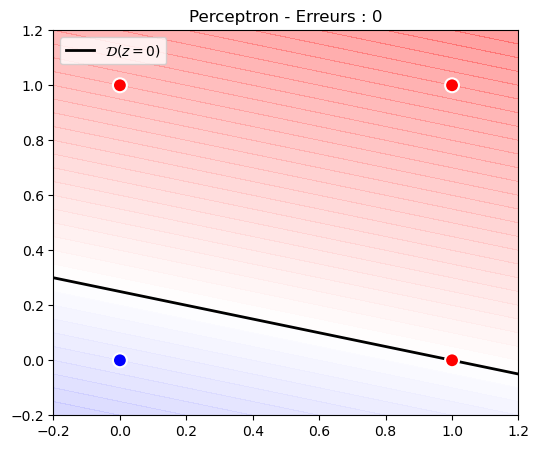
\includegraphics[height=0.8\linewidth]{Images/droite06}
				\label{fig:droite06}
				\caption*{Porte OU}
			\end{figure}			
		\end{column}
	\end{columns}	
\end{frame}

\subsection[Neurone mathématique]{Neurone mathématique}

\begin{frame}{Classe prédite par le Perceptron}
	Pour une observation $i$ donnée, en considérant l'augmentation $x^{(i)} = (x_1^{(i)}, x_2^{(i)}, \cdots, x_p^{(i)}, 1)$ organisée dans un vecteur ligne $x^{(i)} \in \mathcal{M}_{1,p+1}(\R),$  quand l'espace des entrées est p-dimensionnel: $\mathcal{X} \subset \R^p$, on peut écrire la classe prédite $y^{(i)}$ à partir des caractéristiques d'entrée et des coefficients de la droite arrangés en colonne $w = (w_1, w_2, \cdots, w_p, w_{p+1})^T$ comme suit:
	
	\begin{equation*}
		y^{(i)} = \sign{x^{(i)} w}
	\end{equation*}
	
	\pause
	On peut représenter le signe de la quantité $z$ en utilisant la fonction d'Heaviside $\sigma_h: \R \to \{0, 1\}$, la formulation devient alors:
	
	\begin{equation*}
		y^{(i)} = \heaviside{x^{(i)} w}
	\end{equation*}
	
\end{frame}

\begin{frame}{Similarité avec la régression logistique}
	Le Perceptron de Rosenblatt prédit la classe $y^{(i)}$ avec:
	
	\begin{equation*}
		y^{(i)} = \heaviside{x^{(i)} w}
	\end{equation*}
	
	La régression logistique utilise la fonction logistique $\sigma: \R \to ]0, 1[$ à la place de la fonction d'Heaviside:
	
	\begin{equation*}
		y^{(i)} = \logistic{x^{(i)} w}
	\end{equation*}
\end{frame}


\begin{frame}{Reformulation de l'algorithme du Perceptron}
	Sans considérer une augmentation de $x$, on peut simplement écrire $x^{(i)} = (x_1^{(i)}, x_2^{(i)}, \cdots, x_p^{(i)})$. Une formulation équivalente du Perceptron est alors:
	
	\begin{equation*}
		y^{(i)} = \heaviside{x^{(i)} w + w_{p+1}}
	\end{equation*}
	
	Qu'il est plus courant d'écrire:
	
	\begin{equation*}
		y^{(i)} = \heaviside{x^{(i)} w + b}
	\end{equation*}
	
	Où $w$ est appelé \textbf{poids} du Perceptron et $b$ est appelé \textbf{biais} du perceptron.
	
	
	
\end{frame}

\begin{frame}{Anatomie du neurone artificiel de Rosenblatt}
	\begin{center}
		\begin{tikzpicture}[x=1.2cm, y=1cm, >=Stealth]
			
			% --- 1. Entrées (Inputs) ---
			\node[input] (x1) at (0, 2) {$x_1^{(i)}$};
			\node[input] (x2) at (0, 1) {$x_2^{(i)}$};
			\node (xdots) at (0, 0.2) {$\vdots$};
			\node[input] (xn) at (0, -0.7) {$x_p^{(i)}$};
			
			\node[anchor=south, font=\tiny\bfseries] at (x1.north) {Signaux};
			
			% --- 2. Le Soma (Somme + Activation) ---
			% Bloc de Somme
			\node[neuron] (sum) at (3, 0.6) {$\displaystyle \sum$};
			
			% Bloc d'Activation (Heaviside)
			\node[neuron] (act) at (5, 0.6) {};
			
			% Dessin de la marche d'Heaviside à l'intérieur du cercle
			\draw[thick, blue] (4.75, 0.45) -- (5, 0.45) -- (5, 0.75) -- (5.25, 0.75);
			\node[anchor=north, font=\tiny, text=blue] at (act.south) {Heaviside};
			
			% --- 3. Le Biais ---
			\node[input, fill=green!10, draw=green!60!black] (b) at (3, 2.3) {$b$};
			\draw[->, green!60!black, thick] (b) -- (sum) node[midway, right, bias] {+1};
			\node[anchor=west, font=\tiny, green!60!black] at (b.east) {Biais};
			
			% --- 4. Connexions avec Poids ---
			\draw[->] (x1) -- (sum) node[pos=0.4, above, weight] {$w_1$};
			\draw[->] (x2) -- (sum) node[pos=0.4, above, weight] {$w_2$};
			\draw[->, dashed, gray] (xdots) -- (sum);
			\draw[->] (xn) -- (sum) node[pos=0.4, below, weight] {$w_p$};
			
			% --- 5. Transfert interne ---
			\draw[->, thick] (sum) -- (act) node[midway, above, font=\tiny] {$z^{(i)}$};
			
			% --- 6. Sortie (Output) ---
			\node (y) at (7, 0.6) {$y^{(i)}$};
			\draw[->, thick] (act) -- (y);
			
			% --- Annotations mathématiques ---
			\node[anchor=north, font=\scriptsize, text=gray] at (sum.south) {
				$z^{(i)} = \sum_{j=1}^p w_j x_j^{(i)} + b$
			} ;
			
%			\node[anchor=west, font=\scriptsize] at (y.east) {
%				$y^{(i)} = \begin{cases} 1 & \text{si } z^{(i)} > 0 \\ 0 & \text{sinon} \end{cases}$
%			};
			
			% --- Labels de zones ---
			\draw[dashed, gray!40] (2, -1.5) -- (2, 3);
			\node[font=\tiny, gray] at (1, -1.3) {Synapses};
			\node[font=\tiny, gray] at (4, -1.3) {Soma (Corps cellulaire)};
			
		\end{tikzpicture}
	\end{center}
	
	Le perceptron de Rosenblatt (1958) est constitué:
	
	\begin{itemize}
		\item D'une \textbf{linéarité:} Une simple somme pondérée des entrées à laquelle on ajoute un biais (seuil d'activation).
		\item D'une \textbf{fonction de seuil:} la fonction d'Heaviside qui représente la nature "Tout ou Rien" de l'activation d'un neurone humain. 
	\end{itemize}
\end{frame}

\begin{frame}{Limites du Perceptron}
	\begin{itemize}
		\item Comme discuté en introduction, le Perceptron n'est pas capable de résoudre des problèmes de classification qui ne sont pas \textbf{linéairement séparables}, c'est la raison pour laquelle il est tombé dans l'oubli pendant près de 30 ans (avant la découverte de l'algorithme de la rétro-propagation du gradient).
		\item A l'époque du Perceptron, la \textbf{régression logistique} (qui dispose mathématiquement d'une formulation très similaire) était déjà connue. Mais ces outils étaient utilisés dans différents domaines. La régression logistique était utilisée dans le domaine médical pour des analyses statistiques et le Perceptron était avant tout un algorithme censé démontrer la nature calculatoire du cerveau humain.
	\end{itemize}
	
\end{frame}
